\subsection{标量磁场输入与控制插入}

前述实验表明预测步长与物理基线须协同选定；进入受控应用后，外部控制磁场的离散插入方式同样影响精度与功交换。本节将步内、步后与生成函数控制的设想具体化为同一磁势输入的三种物理实例，采用固定增益反馈考察显式物理模型的跟踪表现。沿用式\eqref{eq:learning-model}的显式两模态梁，设横向控制磁场比$u=B_y/B_0$、控制势$V_u=-u\sin\vartheta$（$\vartheta=d^TX$），使标量输入通过$u\,d\cos\vartheta$耦合驱动两模态。与$u$功率共轭的无量纲端口输出及速度为
\begin{equation}
 s(x)=\sin\vartheta,\qquad
 v(x)=\cos\vartheta\,d^T\operatorname{diag}(\nu)Y,
 \label{eq:control-port}
\end{equation}
对应物理输入功率$E_0\omega_0uv$。评测复用全部五个种子的测试初值块（共40条轨迹），公共可行参考由零初态在平滑输入
\[
 u_{\rm ref}(\tau)=0.05\bigl[1-e^{-(\tau/(0.25\omega_0))^2}\bigr]
                    \sin(0.85\tau)
\]
（平滑起始尺度$0.25\,\mathrm s$）下经DOP853积分生成。每步起点采样状态并按零阶保持施加同一反馈律：
\begin{equation}
\begin{aligned}
 u_k=\operatorname{clip}_{[-0.2,0.2]}\bigl\{
 &u_{\rm ref}(\tau_k)-[s(x_k)-s(x_{{\rm ref},k})]\\
 &-0.5[v(x_k)-v(x_{{\rm ref},k})]\bigr\},
\end{aligned}
\label{eq:control-law}
\end{equation}
上限$|u_k|\leq0.2$对应$B_0=0.03\,\mathrm T$时的$|B_y|\leq6\,\mathrm{mT}$。围绕自由保守中点步$\Phi_h^0$，由二类生成函数$S_\ell=X^T\widetilde Y-\ell u\sin(d^TX)$构造控制势精确冲量
\[
 K_\ell^u(X,Y)=\bigl(X,\,Y+\ell u d\cos(d^TX)\bigr),
\]
对比步内受控中点（I）、步后完整冲量（II）与对称半冲量分裂（III）三种一步映射：
\begin{equation}
 \begin{aligned}
 \Psi_{\rm I}&=\mathcal M_h^u,\qquad
 \Psi_{\rm II}=K_h^u\circ\Phi_h^0,\\
 \Psi_{\rm III}&=K_{h/2}^u\circ\Phi_h^0\circ K_{h/2}^u.
 \end{aligned}
 \label{eq:control-maps}
\end{equation}
方案III采用经典Strang对称分裂\citep{Strang1968}，其构造和分裂精度理论归于原文献。II的步后修正限定为物理控制势产生的动量冲量；III由控制势子流与自由中点步对称组合得到，区别于任意全状态残差修正以及在原生成函数梯度中直接追加控制项。$u=0$时三者退化为同一自由步，二次能量与线性控制势极限下I与III严格重合。

\begin{table*}[t]
\centering\small
\caption{同一磁场预算下的控制插入比较。误差为五个初值种子块的均值与样本标准差；代表步长为$h=h_0$。}
\label{tab:control}
\begin{tabular}{lrrrrr}
\toprule
方案 & 输入响应阶 & 杆端RMSE (mm) & 后半时域RMSE (mm) & $\int u^2\,dt$ (s) & 最大$|B_y|$ (mT) \\
\midrule
无控制 & --- & $1.3312\pm0.1723$ & $1.3320\pm0.1732$ & $0.000000\pm0.000000$ & 0.0000 \\
I & 2.0000 & $0.7453\pm0.1271$ & $0.5212\pm0.0901$ & $0.013067\pm0.000587$ & 5.4021 \\
II & 1.0245 & $0.7486\pm0.1275$ & $0.5260\pm0.0908$ & $0.013062\pm0.000592$ & 5.4024 \\
III & 2.0000 & $0.7453\pm0.1271$ & $0.5212\pm0.0901$ & $0.013067\pm0.000587$ & 5.4021 \\
\bottomrule
\end{tabular}
\par\smallskip\begin{minipage}{0.97\textwidth}\footnotesize I为步内受控中点，II为自由中点后完整势冲量，III为对称半冲量组合。闭环均使用同一标量端口反馈、增益及$|u|\leq0.2$，对应$|B_y|\leq6$ mT；各方案沿自身状态采样，实际输入序列不同。观察阶来自零初值、共同平滑输入的最细两档确定性响应，不包含种子统计；跟踪误差来自全部40个初值，另含输入保持误差。种子仅划分初值，不代表独立控制器训练。\end{minipage}
\end{table*}

\begin{figure*}[t]
\centering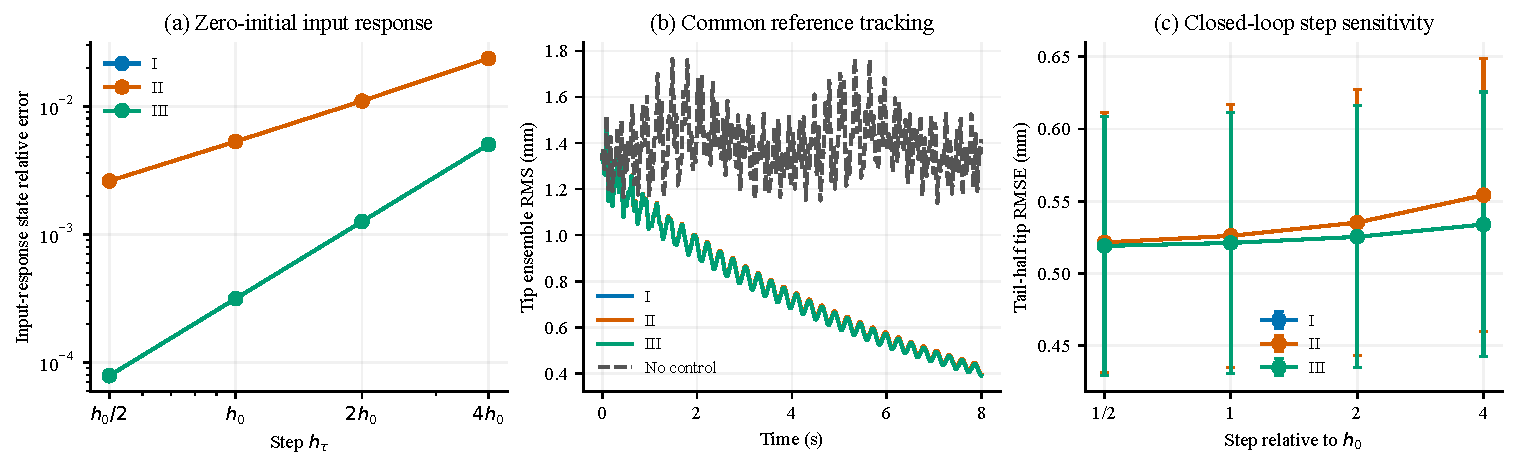
\includegraphics[width=0.98\textwidth]{control_comparison.pdf}
\caption{三种磁场载荷插入的数值比较。左：零初值、同一平滑输入的状态误差；中：$h_0$下40条轨迹相对公共参考的杆端误差，曲线为各时刻的集合RMS，I与III近乎重合；右：后半时域杆端RMSE的步长敏感性，误差线为五个初值块的样本标准差。中图的集合RMS与表中先逐轨迹求RMSE再平均的口径不同。}
\label{fig:control}
\end{figure*}

\subsection{精度、跟踪与结构比较}

在基准步长$h_0=0.009999813692$下取$4h_0$、$2h_0$、$h_0$与$h_0/2$四档步长（时域$7.995\,\mathrm s$；DOP853容差$10^{-12}$、$10^{-14}$，加密容差变化不超过$1.01\times10^{-11}$）。40条非零初值开环轨迹受自由模态相位误差主导，最细两档均呈近二阶表观收敛；改考察零初值在公共输入$u_{\rm ref}$驱动下的纯受迫响应以分离插入误差（图\ref{fig:control}左），则I与对称方案III的观察阶约为$2.0000$，步后方案II由$1.1041$趋至$1.0245$，与一阶分裂误差相符。这一阶数比较限于所测零初值、平滑外加输入的开环响应；闭环相对连续反馈参考的误差还包含起点采样保持的影响。

步长$h_0$的闭环结果见表\ref{tab:control}及图\ref{fig:control}中、右图（逐轨迹求RMSE，在每块8条轨迹内平均后再跨五个初值块统计）。反馈使杆端跟踪RMSE由无控制的$1.3312\pm0.1723\,\mathrm{mm}$降至I的$0.7453\pm0.1271$、II的$0.7486\pm0.1275$及III的$0.7453\pm0.1271\,\mathrm{mm}$（后半时域约$0.5212$、$0.5260$和$0.5212\,\mathrm{mm}$）；完整状态误差由$3.3027$降至$1.6033$、$1.6104$和$1.6033$，端口RMSE由$0.03176$降至约$0.0131$，说明所设反馈降低了跟踪误差，有限时域内仍保留状态偏差。峰值输入$0.18129<0.2$，未触发饱和；I与III的跟踪表现及$\int u^2dt$近乎相同。在$h_0$下，II减I的杆端RMSE配对差为$3.2935\pm0.4552\,\mu\mathrm m$，五个初值块中方向均相同。这是当前模型、反馈律和时域内幅度较小的跟踪收益，不能单凭这一差值确定普遍优越性。



在首块48组一步映射上（中点求解残差均小于$1.3\times10^{-16}$），固定外生$u_k$时$\|D\Psi^TJD\Psi-J\|_F$最大仅$4.72\times10^{-16}$，计入反馈导数$du_k/dx_k$后升至$0.00540$--$0.02106$（解析与差分一致），表明外生输入保辛不直接延伸至闭环映射；按保持功$W_k=u_k[s(x_{k+1})-s(x_k)]$核验基能量$h_*$的累计变化，所测时域内最大归一化功—能残差在$h_0$下分别为I的$6.25\times10^{-8}$、III的$4.19\times10^{-8}$和II的$5.16\times10^{-3}$。该诊断显示本工况中步后完整冲量的功交换离散偏差较大，不构成一般反馈系统的能量稳定性保证。

\subsection{对预测与受控应用的启示}

上述结果将物理基线、相位分辨尺度与控制插入联系起来：预测指标、开环精度、闭环跟踪和功交换分别反映不同误差来源。前述比较使用完整显式模型；为进一步检验已学残差的实际作用，下面将名义模型遗漏的磁势力与网络估计联系到同一物理端口。
